\section{Results}
\label{sec:results}

\paragraph{Protocol.} Every number below is produced by \code{benchmark.py} and turned into tables
and figures by \code{make\_figures.py}. The headline and ablation experiments use 5 seeds
(0--4); all other sweeps use 3 seeds (0--2). Each seed redraws the balanced sample, the
80/20 stratified split, the preprocessing, the tuning and the test. With the default 2{,}000
samples the test set has 400 flows, so one flow is 0.25 accuracy points. ``Sig.'' is the number
of seeds in which the exact McNemar test (QSVM vs.\ RBF-SVM, same test flows) gives $p<0.05$.
Unless stated otherwise, the improved protocol is used: deduplication on the task label,
train-only preprocessing with the signed log transform, and 5-fold CV tuning of
$(\alpha, C)$ for the QSVM and $(C,\gamma)$ for the RBF-SVM with the same $C$ grid.

\subsection{Headline: the same circuits under the original and the improved protocol}

Table~\ref{tab:headline} runs the paper's three methods (the ZZ entangling map with the
paper's circuit settings, the separable $R_x$ map and its 1024-shot version) under both
protocols, plus a 16-qubit, 2-repetition ZZ circuit. Figure~\ref{fig:headline} shows the same
data.

\begin{table}[H]
\centering\small
\caption{Test accuracy (\%) and QSVM macro-F1 (\%), mean $\pm$ std over 5 seeds. ``Legacy'' is
the original protocol (\code{--legacy}); ``improved'' is the corrected one. ZZ uses the paper's
settings: 8 qubits / 2 reps (binary) and 16 qubits / 1 rep (multiclass). $R_x$ uses 16 qubits.}
\label{tab:headline}
\resizebox{\linewidth}{!}{%
\begin{tabular}{lllcccc}
\toprule
Task & Method & Protocol & QSVM acc. & RBF-SVM acc. & QSVM macro-F1 & Sig. \\
\midrule
binary & ZZ entangling (paper circuit) & legacy & 99.50 $\pm$ 0.32 & 97.35 $\pm$ 0.25 & 99.50 $\pm$ 0.32 & 5/5 \\
binary & ZZ entangling (paper circuit) & improved & 99.60 $\pm$ 0.41 & 99.55 $\pm$ 0.29 & 99.60 $\pm$ 0.41 & 0/5 \\
binary & Analytical $R_x$ (separable) & legacy & 98.35 $\pm$ 0.12 & 98.60 $\pm$ 0.41 & 98.35 $\pm$ 0.12 & 0/5 \\
binary & Analytical $R_x$ (separable) & improved & 99.50 $\pm$ 0.32 & 99.50 $\pm$ 0.27 & 99.50 $\pm$ 0.32 & 0/5 \\
binary & Sampling, 1024 shots ($R_x$) & legacy & 98.30 $\pm$ 0.10 & 98.60 $\pm$ 0.41 & 98.30 $\pm$ 0.10 & 0/5 \\
binary & Sampling, 1024 shots ($R_x$) & improved & 99.30 $\pm$ 0.62 & 99.50 $\pm$ 0.27 & 99.30 $\pm$ 0.62 & 0/5 \\
binary & ZZ, 16 qubits, 2 reps & improved & 99.60 $\pm$ 0.25 & 99.50 $\pm$ 0.27 & 99.60 $\pm$ 0.25 & 0/5 \\
\midrule
multiclass & ZZ entangling (paper circuit) & legacy & 95.70 $\pm$ 0.56 & 88.85 $\pm$ 1.12 & 95.68 $\pm$ 0.59 & 5/5 \\
multiclass & ZZ entangling (paper circuit) & improved & 90.85 $\pm$ 0.85 & 91.05 $\pm$ 0.95 & 90.85 $\pm$ 0.86 & 0/5 \\
multiclass & Analytical $R_x$ (separable) & legacy & 91.70 $\pm$ 2.54 & 88.85 $\pm$ 1.12 & 91.60 $\pm$ 2.55 & 2/5 \\
multiclass & Analytical $R_x$ (separable) & improved & 91.05 $\pm$ 0.24 & 91.05 $\pm$ 0.95 & 91.10 $\pm$ 0.22 & 0/5 \\
multiclass & Sampling, 1024 shots ($R_x$) & legacy & 91.35 $\pm$ 1.30 & 88.85 $\pm$ 1.12 & 91.27 $\pm$ 1.32 & 2/5 \\
multiclass & Sampling, 1024 shots ($R_x$) & improved & 88.10 $\pm$ 0.41 & 91.05 $\pm$ 0.95 & 88.16 $\pm$ 0.37 & 2/5 \\
multiclass & ZZ, 16 qubits, 2 reps & improved & 91.20 $\pm$ 0.84 & 91.05 $\pm$ 0.95 & 91.22 $\pm$ 0.86 & 0/5 \\

\bottomrule
\end{tabular}}
\end{table}

\begin{figure}[H]
\centering
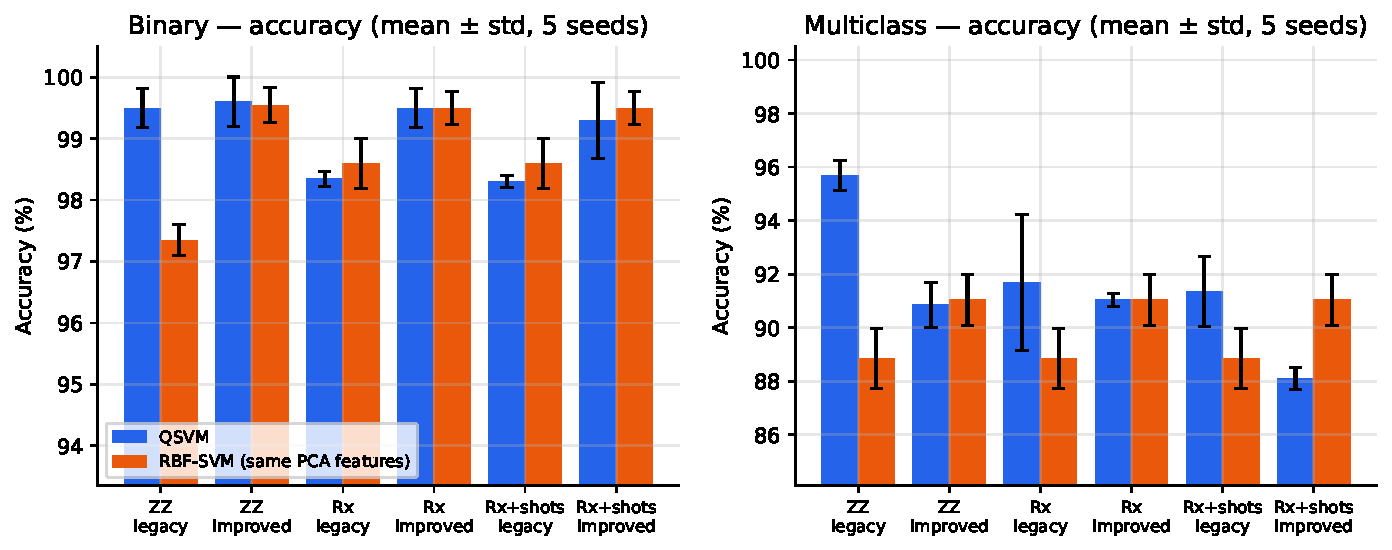
\includegraphics[width=\linewidth]{figures/headline.pdf}
\caption{Accuracy of the QSVM (blue) and the RBF-SVM on the same PCA features (orange) under
both protocols. Error bars: standard deviation over 5 seeds.}
\label{fig:headline}
\end{figure}

\paragraph{The original protocol reproduces the paper's pattern.} Under \code{--legacy} the ZZ
QSVM beats the RBF-SVM by $+2.15$ points (binary) and $+6.85$ points (multiclass), significant in
5/5 seeds both times. Summed over the five seeds, the QSVM is right where the RBF-SVM is wrong on
46 binary flows and the reverse happens on 3; in multiclass the counts are 172 and 35. The
paper's observation is therefore real \emph{under its protocol}.

\paragraph{The improved protocol removes the gap.} With the same circuits, the differences shrink
to $+0.05$ (binary) and $-0.20$ points (multiclass), and no seed is significant. Pooled over the
seeds, the discordant counts are 2 vs.\ 1 (binary) and 19 vs.\ 23 (multiclass). The QSVM did not
become worse in binary mode (99.50\% $\to$ 99.60\%); the RBF-SVM became much better
(97.35\% $\to$ 99.55\%; multiclass 88.85\% $\to$ 91.05\%). The same holds for the 16-qubit,
2-repetition circuit (99.60 vs.\ 99.50; 91.20 vs.\ 91.05) and for the separable $R_x$ kernel,
which ties the RBF-SVM exactly in both tasks.

\paragraph{Shot noise.} In binary mode the 1024-shot $R_x$ kernel is within noise of the exact
one. In multiclass mode it costs about 3 points (88.10\% vs.\ 91.05\% exact), and the RBF-SVM is
significantly better in 2/5 seeds. Section~\ref{sec:res-shots} explains why this happens at 16
qubits but not at 8.

\subsection{Ablation: which fix changes what}

Table~\ref{tab:ablation} and Figure~\ref{fig:ablation} add the fixes one at a time to the ZZ
pipeline with the paper's circuit settings, starting from the original protocol.

\begin{table}[H]
\centering\small
\caption{Cumulative ablation (5 seeds). ``Overlap'' is the fraction of test flows with an exact
copy in the training set. Gap = QSVM $-$ RBF-SVM accuracy in points.}
\label{tab:ablation}
\begin{tabular}{llccccc}
\toprule
Task & Step & Overlap & QSVM acc. & RBF-SVM acc. & Gap & Sig. \\
\midrule
binary & Original protocol & 28.4\% & 99.50 $\pm$ 0.32 & 97.35 $\pm$ 0.25 & +2.15 & 5/5 \\
binary & + remove duplicates & 0.0\% & 98.85 $\pm$ 0.49 & 96.15 $\pm$ 0.51 & +2.70 & 4/5 \\
binary & + train-only scaling & 0.0\% & 98.65 $\pm$ 0.34 & 96.40 $\pm$ 0.89 & +2.25 & 3/5 \\
binary & + log transform & 0.0\% & 99.15 $\pm$ 0.46 & 99.40 $\pm$ 0.68 & -0.25 & 0/5 \\
binary & + CV tuning ($\alpha$, $C$, $\gamma$) & 0.0\% & 99.60 $\pm$ 0.41 & 99.55 $\pm$ 0.29 & +0.05 & 0/5 \\
\midrule
multiclass & Original protocol & 48.6\% & 95.70 $\pm$ 0.56 & 88.85 $\pm$ 1.12 & +6.85 & 5/5 \\
multiclass & + remove duplicates & 0.8\% & 89.20 $\pm$ 1.02 & 87.55 $\pm$ 1.44 & +1.65 & 2/5 \\
multiclass & + train-only scaling & 0.8\% & 88.40 $\pm$ 1.22 & 87.35 $\pm$ 1.45 & +1.05 & 2/5 \\
multiclass & + log transform & 0.8\% & 91.40 $\pm$ 0.78 & 90.20 $\pm$ 0.58 & +1.20 & 0/5 \\
multiclass & + CV tuning ($\alpha$, $C$, $\gamma$) & 0.8\% & 90.85 $\pm$ 0.85 & 91.05 $\pm$ 0.95 & -0.20 & 0/5 \\

\bottomrule
\end{tabular}
\end{table}

\begin{figure}[H]
\centering
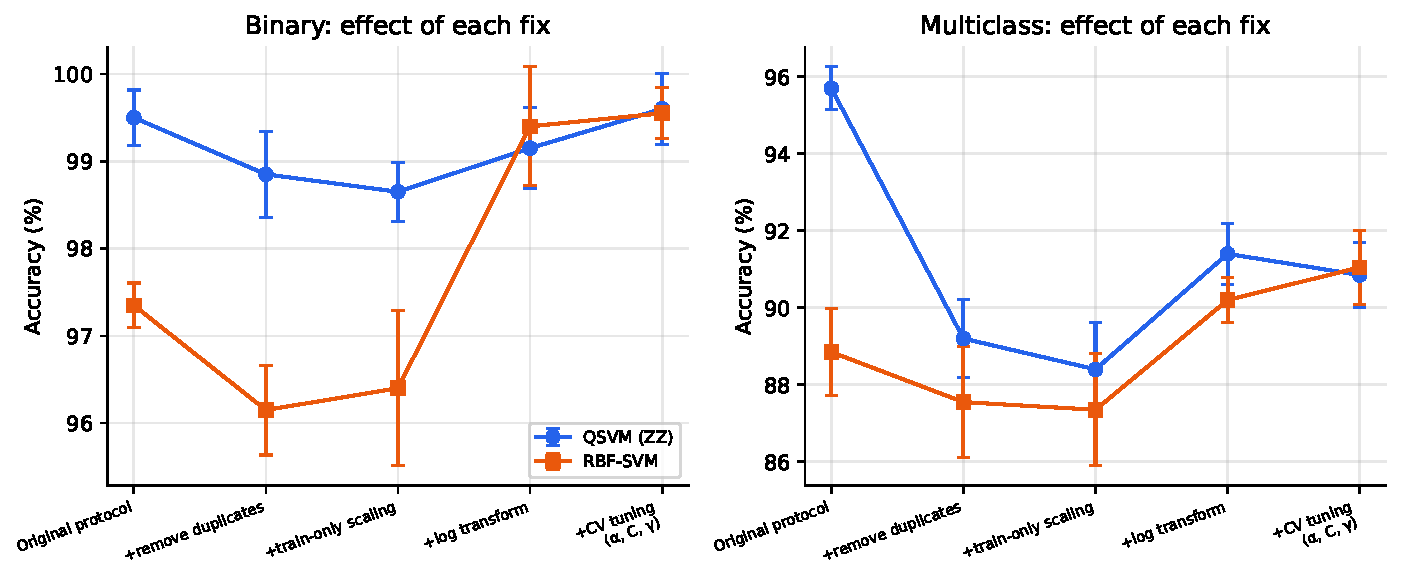
\includegraphics[width=0.95\linewidth]{figures/ablation.pdf}
\caption{Effect of each fix on QSVM and RBF-SVM accuracy (mean $\pm$ std, 5 seeds).}
\label{fig:ablation}
\end{figure}

\begin{itemize}
\item \textbf{Removing duplicates} is the largest single effect in multiclass mode. The QSVM
      loses 6.5 points (95.70\% $\to$ 89.20\%) and the gap shrinks from $+6.85$ to $+1.65$. The
      QSVM profited more from duplicates than the RBF-SVM: with $\alpha=1$ its kernel is close to
      the identity, so a test flow with a training twin gets $K=1$ to that twin and almost 0 to
      everything else, which is pure memorisation. In binary mode the overlap was smaller (28\%)
      and both models lose 0.65--1.2 points.
\item \textbf{Train-only scaling} changes little on its own ($\le$0.8 points). It is a
      correctness fix, not a performance one.
\item \textbf{The log transform} closes the binary gap. The RBF-SVM jumps by 3.0 points
      (96.40\% $\to$ 99.40\%) and the gap goes from $+2.25$ to $-0.25$. Under linear min--max
      scaling the heavy-tailed features squeeze most flows into a small corner of each PCA
      component (Figure~\ref{fig:skew}), and the RBF-SVM with a default $\gamma$ suffers from this
      much more than the QSVM. Part of the original ``advantage'' was therefore an encoding
      artefact that hurt the baseline.
\item \textbf{CV tuning} gives the last few tenths of a point and removes the remaining multiclass
      gap ($+1.20 \to -0.20$).
\end{itemize}

\subsection{All metrics for the improved ZZ pipeline}

\begin{table}[H]
\centering\small
\caption{All metrics (\%), improved protocol, ZZ with the paper's circuit settings, 5 seeds.
FAR: benign flows flagged as attacks. DR: attack flows flagged as some attack.}
\label{tab:metrics}
\resizebox{\linewidth}{!}{%
\begin{tabular}{llccccccc}
\toprule
Task & Model & Accuracy & Bal.\ acc. & Macro-F1 & MCC & AUC & FAR & DR \\
\midrule
binary & QSVM ZZ (tuned) & 99.60 $\pm$ 0.41 & 99.60 $\pm$ 0.41 & 99.60 $\pm$ 0.41 & 99.20 $\pm$ 0.81 & 99.92 $\pm$ 0.15 & 0.30 $\pm$ 0.40 & 99.50 $\pm$ 0.63 \\
binary & RBF-SVM (tuned) & 99.55 $\pm$ 0.29 & 99.55 $\pm$ 0.29 & 99.55 $\pm$ 0.29 & 99.10 $\pm$ 0.58 & 99.92 $\pm$ 0.14 & 0.40 $\pm$ 0.37 & 99.50 $\pm$ 0.63 \\
binary & Random Forest & 99.70 $\pm$ 0.29 & 99.70 $\pm$ 0.29 & 99.70 $\pm$ 0.29 & 99.40 $\pm$ 0.58 & 99.99 $\pm$ 0.02 & 0.10 $\pm$ 0.20 & 99.50 $\pm$ 0.63 \\
\midrule
multiclass & QSVM ZZ (tuned) & 90.85 $\pm$ 0.85 & 90.86 $\pm$ 0.85 & 90.85 $\pm$ 0.86 & 89.05 $\pm$ 1.01 & 98.71 $\pm$ 0.15 & 1.79 $\pm$ 1.46 & 98.62 $\pm$ 0.73 \\
multiclass & RBF-SVM (tuned) & 91.05 $\pm$ 0.95 & 91.06 $\pm$ 0.95 & 91.07 $\pm$ 0.98 & 89.29 $\pm$ 1.14 & 98.73 $\pm$ 0.28 & 2.09 $\pm$ 2.02 & 98.98 $\pm$ 0.67 \\
multiclass & Random Forest & 93.10 $\pm$ 0.49 & 93.11 $\pm$ 0.49 & 93.11 $\pm$ 0.48 & 91.74 $\pm$ 0.58 & 99.03 $\pm$ 0.07 & 2.09 $\pm$ 1.52 & 99.46 $\pm$ 0.29 \\

\bottomrule
\end{tabular}}
\end{table}

Table~\ref{tab:metrics} confirms the headline with every metric: the QSVM and the RBF-SVM are
within one standard deviation of each other on accuracy, balanced accuracy, macro-F1, MCC, AUC,
false-alarm rate and detection rate. The Random Forest on all 49 raw features is the best model
in both tasks (99.70\% binary, 93.10\% multiclass). The kernel models only see at most 16 PCA
components, and that compression has a cost.

\paragraph{Where the multiclass errors are.} Summed over the five seeds, the QSVM's per-class
recall is BENIGN 98.2\%, UDP 95.5\%, Syn 92.5\%, LDAP 89.2\%, MSSQL 87.4\% and Portmap 82.3\%.
The RBF-SVM's recalls are within 1 point of these for every class. Almost all errors are
confusions between the three reflection attacks (LDAP $\leftrightarrow$ MSSQL $\leftrightarrow$
Portmap), plus Portmap flows predicted as BENIGN or Syn. These are the classes whose flows are
70--94\% duplicates in the raw file, so they are the ones that looked easiest under the original
protocol. The Random Forest gains most on MSSQL (+4.5), Portmap (+4.5) and UDP (+3.3).

\subsection{Bandwidth $\alpha$}

Table~\ref{tab:bandwidth} and Figure~\ref{fig:bandwidth} fix $\alpha$ (tuning only $C$) for the
ZZ map with 2 repetitions at 8 and 16 qubits.

\begin{figure}[H]
\centering
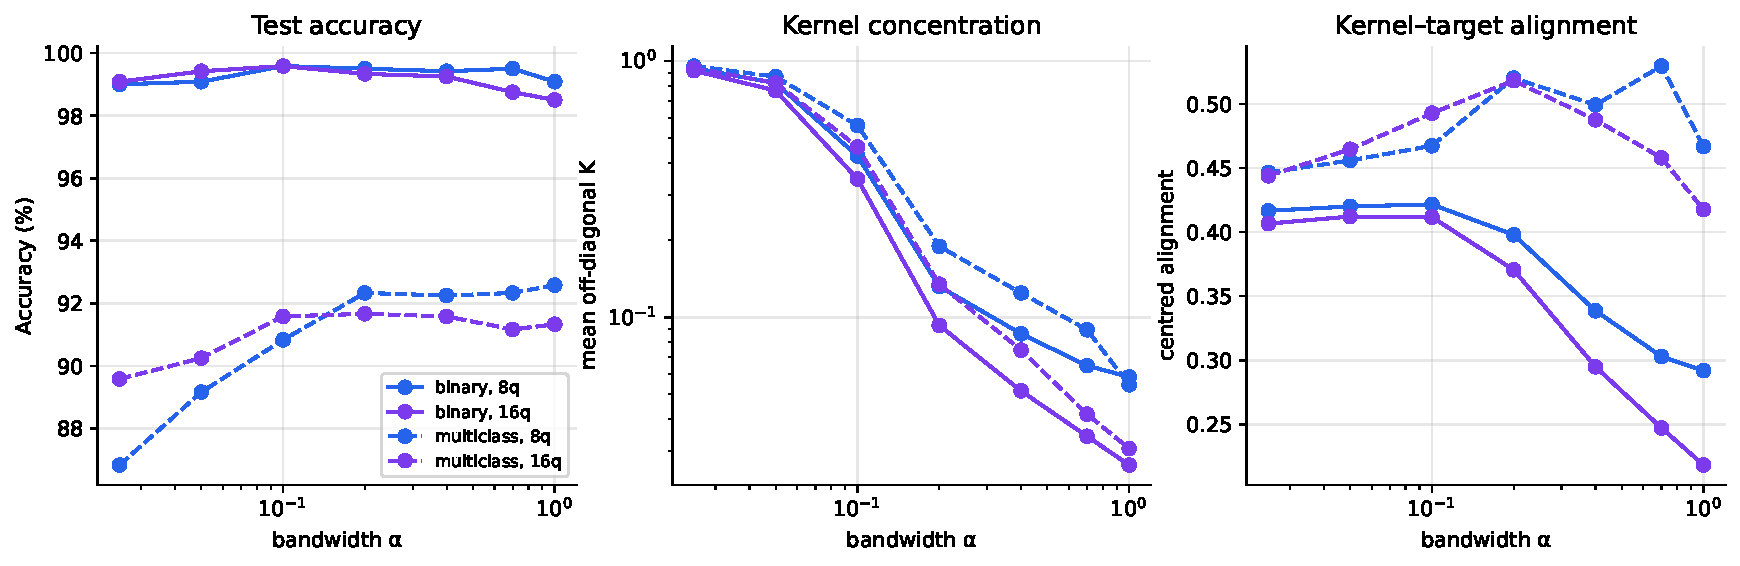
\includegraphics[width=\linewidth]{figures/bandwidth.pdf}
\caption{Test accuracy, mean off-diagonal kernel value and centred kernel--target alignment as
functions of $\alpha$ (ZZ map, 2 reps, 3 seeds).}
\label{fig:bandwidth}
\end{figure}

\begin{table}[H]
\centering\small
\caption{Bandwidth sweep (3 seeds): QSVM accuracy (\%), mean off-diagonal training kernel value,
and centred kernel--target alignment.}
\label{tab:bandwidth}
\begin{tabular}{lcccccc}
\toprule
Task & Qubits & $\alpha$ & QSVM acc. & Mean off-diag.\ $K$ & Alignment \\
\midrule
binary & 8 & 0.025 & 99.00 & 9.38e-01 & 0.417 \\
binary & 8 & 0.05 & 99.08 & 8.19e-01 & 0.420 \\
binary & 8 & 0.1 & 99.58 & 4.26e-01 & 0.422 \\
binary & 8 & 0.2 & 99.50 & 1.32e-01 & 0.398 \\
binary & 8 & 0.4 & 99.42 & 8.62e-02 & 0.339 \\
binary & 8 & 0.7 & 99.50 & 6.47e-02 & 0.303 \\
binary & 8 & 1 & 99.08 & 5.85e-02 & 0.292 \\
binary & 16 & 0.025 & 99.08 & 9.17e-01 & 0.407 \\
binary & 16 & 0.05 & 99.42 & 7.66e-01 & 0.412 \\
binary & 16 & 0.1 & 99.58 & 3.46e-01 & 0.412 \\
binary & 16 & 0.2 & 99.33 & 9.29e-02 & 0.371 \\
binary & 16 & 0.4 & 99.25 & 5.16e-02 & 0.295 \\
binary & 16 & 0.7 & 98.75 & 3.43e-02 & 0.247 \\
binary & 16 & 1 & 98.50 & 2.65e-02 & 0.218 \\
multiclass & 8 & 0.025 & 86.83 & 9.56e-01 & 0.446 \\
multiclass & 8 & 0.05 & 89.17 & 8.69e-01 & 0.456 \\
multiclass & 8 & 0.1 & 90.83 & 5.60e-01 & 0.467 \\
multiclass & 8 & 0.2 & 92.33 & 1.89e-01 & 0.520 \\
multiclass & 8 & 0.4 & 92.25 & 1.24e-01 & 0.499 \\
multiclass & 8 & 0.7 & 92.33 & 8.93e-02 & 0.530 \\
multiclass & 8 & 1 & 92.58 & 5.45e-02 & 0.467 \\
multiclass & 16 & 0.025 & 89.58 & 9.37e-01 & 0.444 \\
multiclass & 16 & 0.05 & 90.25 & 8.20e-01 & 0.465 \\
multiclass & 16 & 0.1 & 91.58 & 4.62e-01 & 0.493 \\
multiclass & 16 & 0.2 & 91.67 & 1.34e-01 & 0.518 \\
multiclass & 16 & 0.4 & 91.58 & 7.45e-02 & 0.488 \\
multiclass & 16 & 0.7 & 91.17 & 4.19e-02 & 0.458 \\
multiclass & 16 & 1 & 91.33 & 3.07e-02 & 0.418 \\

\bottomrule
\end{tabular}
\end{table}

\begin{itemize}
\item The mean off-diagonal kernel value falls by more than an order of magnitude from
      $\alpha=0.025$ to $\alpha=1$ (e.g.\ 0.92 $\to$ 0.027 at 16 qubits, binary). This is the
      concentration effect of Section~\ref{sec:conc}, and it is stronger at 16 qubits than at 8.
\item At 16 qubits, accuracy peaks at $\alpha\approx0.1$--0.2 and falls at $\alpha=1$ (binary
      99.58\% $\to$ 98.50\%), and alignment falls with it (0.41 $\to$ 0.22). At 8 qubits the
      kernel concentrates less, so the curve is flatter. Without a bandwidth, the paper's
      16-qubit circuit sits in the worst part of the curve.
\item Very small $\alpha$ also hurts, especially in multiclass mode (86.8\% at 8 qubits,
      $\alpha=0.025$): the kernel approaches the constant 1 and the classes are no longer
      separated.
\item In binary mode, alignment and accuracy peak at the same $\alpha$ ($\approx0.1$); in
      multiclass mode they peak at roughly similar values. The cheap alignment diagnostic (no SVM
      training needed) is therefore a rough guide for choosing $\alpha$, but not a substitute
      for CV.
\end{itemize}

\subsection{Number of qubits}

\begin{figure}[H]
\centering
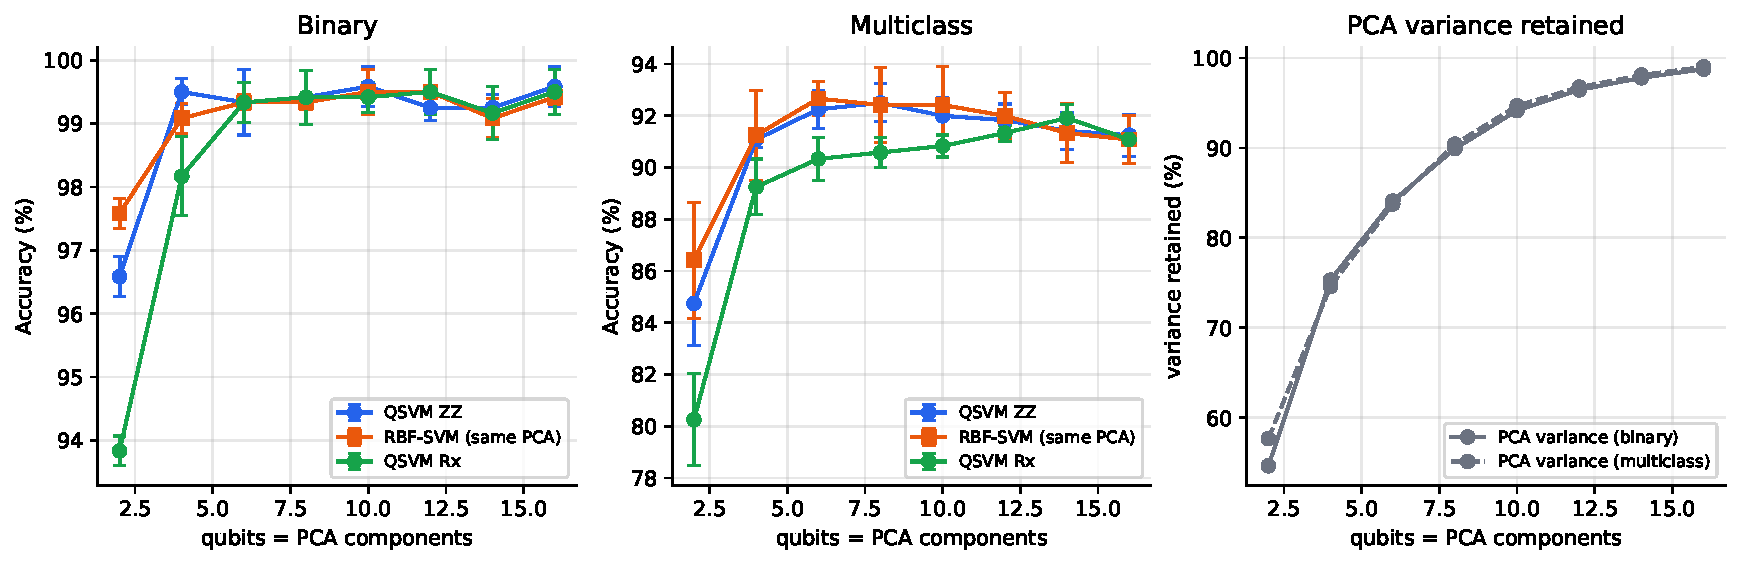
\includegraphics[width=\linewidth]{figures/qubits.pdf}
\caption{Accuracy vs.\ number of qubits (= PCA components) for the ZZ and $R_x$ QSVMs and the
RBF-SVM on the same components, and the PCA variance retained (3 seeds).}
\label{fig:qubits}
\end{figure}

\begin{table}[H]
\centering\small
\caption{Qubit sweep for the ZZ map (2 reps, 3 seeds): PCA variance retained (\%), accuracy (\%),
mean tuned $\alpha$ and geometric difference $g$ against the tuned RBF kernel
($\sqrt{N}=20$).}
\label{tab:qubits}
\begin{tabular}{lcccccc}
\toprule
Task & Qubits & PCA var. & QSVM ZZ & RBF-SVM & Mean $\alpha$ & $g$ \\
\midrule
binary & 2 & 54.6 & 96.58 & 97.58 & 1.000 & 39.36 \\
binary & 4 & 75.3 & 99.50 & 99.08 & 0.333 & 10.26 \\
binary & 6 & 84.1 & 99.33 & 99.33 & 0.400 & 3.75 \\
binary & 8 & 89.9 & 99.42 & 99.33 & 0.333 & 14.49 \\
binary & 10 & 94.2 & 99.58 & 99.50 & 0.233 & 10.14 \\
binary & 12 & 96.4 & 99.25 & 99.50 & 0.133 & 14.06 \\
binary & 14 & 97.8 & 99.25 & 99.08 & 0.133 & 8.97 \\
binary & 16 & 98.8 & 99.58 & 99.42 & 0.100 & 2.22 \\
multiclass & 2 & 57.7 & 84.75 & 86.42 & 1.000 & 31.05 \\
multiclass & 4 & 74.6 & 91.08 & 91.25 & 0.800 & 32.40 \\
multiclass & 6 & 83.7 & 92.25 & 92.67 & 0.800 & 9.77 \\
multiclass & 8 & 90.4 & 92.50 & 92.42 & 0.800 & 17.52 \\
multiclass & 10 & 94.7 & 92.00 & 92.42 & 0.333 & 3.00 \\
multiclass & 12 & 96.8 & 91.83 & 92.00 & 0.233 & 7.86 \\
multiclass & 14 & 98.1 & 91.42 & 91.33 & 0.333 & 2.50 \\
multiclass & 16 & 99.0 & 91.25 & 91.08 & 0.333 & 3.94 \\

\bottomrule
\end{tabular}
\end{table}

Accuracy saturates early: at 4 qubits the binary task is already at 99.5\%, and multiclass
accuracy stops improving at 6--8 qubits (84--90\% PCA variance). From 4 qubits on, the QSVM and
the RBF-SVM are within 0.5 points of each other at every width; only at 2 qubits is the RBF-SVM
1--1.7 points ahead. As the circuit gets wider, the tuned $\alpha$ falls (from 1.0 at 2 qubits
to 0.1--0.33 at 12--16 qubits), which is the tuning compensating for concentration. Adding qubits makes the Hilbert space exponentially larger, but
that does not show up in accuracy.

\subsection{Shot noise}
\label{sec:res-shots}

\begin{figure}[H]
\centering
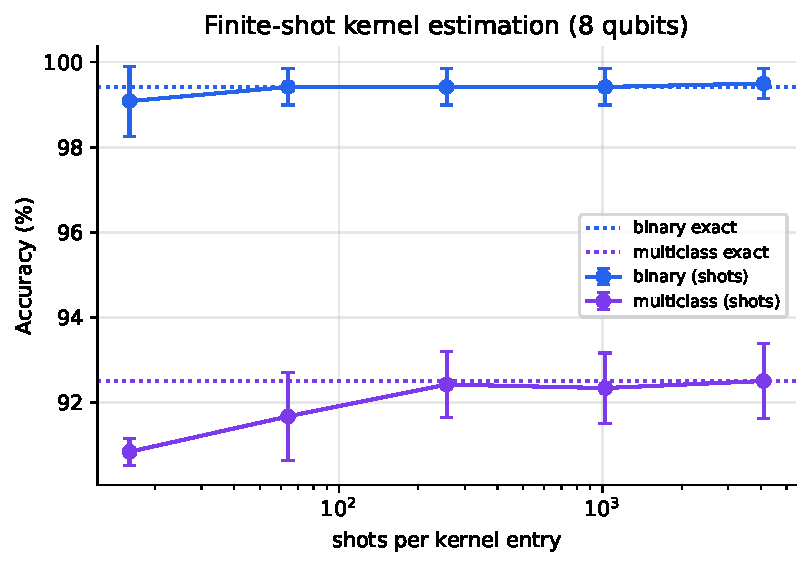
\includegraphics[width=0.6\linewidth]{figures/shots.pdf}
\caption{QSVM accuracy vs.\ shots per kernel entry (ZZ, 8 qubits, 2 reps, 3 seeds). Dotted lines:
exact kernel.}
\label{fig:shots}
\end{figure}

\begin{table}[H]
\centering\small
\caption{Shot sweep, ZZ map, 8 qubits (3 seeds): accuracy (\%) and mean tuned $\alpha$.}
\label{tab:shots}
\begin{tabular}{lccc}
\toprule
Task & Shots & QSVM acc. & Mean $\alpha$ \\
\midrule
binary & 16 & 99.08 $\pm$ 0.82 & 0.533 \\
binary & 64 & 99.42 $\pm$ 0.42 & 0.400 \\
binary & 256 & 99.42 $\pm$ 0.42 & 0.333 \\
binary & 1024 & 99.42 $\pm$ 0.42 & 0.267 \\
binary & 4096 & 99.50 $\pm$ 0.35 & 0.267 \\
binary & exact & 99.42 $\pm$ 0.42 & 0.333 \\
multiclass & 16 & 90.83 $\pm$ 0.31 & 1.000 \\
multiclass & 64 & 91.67 $\pm$ 1.03 & 1.000 \\
multiclass & 256 & 92.42 $\pm$ 0.77 & 1.000 \\
multiclass & 1024 & 92.33 $\pm$ 0.82 & 1.000 \\
multiclass & 4096 & 92.50 $\pm$ 0.89 & 0.800 \\
multiclass & exact & 92.50 $\pm$ 0.74 & 0.800 \\

\bottomrule
\end{tabular}
\end{table}

At 8 qubits, 256 shots per entry already match the exact kernel in both tasks, and even 16
shots cost only 0.3 (binary) and 1.7 points (multiclass). The tuned $\alpha$ moves to larger
values as the shot count falls (binary: 0.27 at 1024--4096 shots, 0.53 at 16). A likely reason
is that larger $\alpha$ pushes most kernel values towards 0, where the binomial variance
$K(1-K)/s$ is small, so CV picks a bandwidth that limits the noise.

The 16-qubit $R_x$ result in Table~\ref{tab:headline} is different: there, 1024 shots cost 3
points in multiclass mode, while in binary mode they cost nothing. With 1024 shots each entry has
a standard deviation of up to $\sqrt{0.25/1024}\approx0.016$. The binary classes are far apart
in kernel space, but the three reflection attacks are separated by small kernel differences that
are apparently of the same order. We have not isolated why the 8-qubit ZZ kernel is robust and
the 16-qubit $R_x$ kernel is not. The practical lesson is that the shot budget needed depends on
the circuit and the task, and has to be measured before trusting a hardware result.

\paragraph{Projecting the noisy kernel onto the PSD cone does not help.} An estimated Gram matrix
is not positive semi-definite. On 1{,}600 multiclass training flows (16 qubits, $R_x$, 1024
shots), the negative eigenvalues sum to between $-83$ and $-319$ depending on $\alpha$, so the
SVM dual is no longer convex. The standard remedy is to clip the negative eigenvalues of the
training kernel to zero~\cite{hubregtsen2022}, available as \code{--psd}. On the multiclass
headline it made results worse in 5/5 seeds (88.10\% $\to$ 84.65\%). Clipping changes only the
training kernel, while the test kernel keeps its noise, so the two no longer describe the same
geometry. The option is therefore off by default.

\subsection{Circuit architecture and feature set}

\begin{table}[H]
\centering\small
\caption{ZZ QSVM accuracy (\%) by number of repetitions and entanglement topology (8 qubits,
3 seeds).}
\label{tab:arch}
\begin{tabular}{llccc}
\toprule
Task & Reps & Linear & Circular & Full \\
\midrule
binary & 1 & 99.25 $\pm$ 0.20 & 99.25 $\pm$ 0.20 & 99.25 $\pm$ 0.41 \\
binary & 2 & 99.42 $\pm$ 0.42 & 99.50 $\pm$ 0.35 & 99.33 $\pm$ 0.24 \\
binary & 3 & 99.42 $\pm$ 0.42 & 99.17 $\pm$ 0.24 & 99.42 $\pm$ 0.12 \\
\midrule
multiclass & 1 & 92.58 $\pm$ 0.66 & 92.50 $\pm$ 0.71 & 92.50 $\pm$ 0.54 \\
multiclass & 2 & 92.50 $\pm$ 0.74 & 92.58 $\pm$ 0.82 & 92.00 $\pm$ 0.35 \\
multiclass & 3 & 92.42 $\pm$ 1.45 & 92.75 $\pm$ 0.89 & 91.92 $\pm$ 0.12 \\

\bottomrule
\end{tabular}
\end{table}

No architecture stands out (Table~\ref{tab:arch}). All nine combinations of 1--3 repetitions and
linear, circular or full entanglement are within 0.35 points of each other in binary mode and
0.85 points in multiclass mode, which is within one standard deviation. More entanglement or more
repetitions, which make the kernel harder to simulate classically, do not make it more accurate
here.

\begin{table}[H]
\centering\small
\caption{Feature set (8 qubits, 3 seeds): accuracy (\%).}
\label{tab:features}
\begin{tabular}{llccc}
\toprule
Task & Feature set & QSVM ZZ & RBF-SVM & Random Forest \\
\midrule
binary & paper (61 listed, 49 non-constant) & 99.42 $\pm$ 0.42 & 99.33 $\pm$ 0.12 & 99.50 $\pm$ 0.20 \\
binary & all numeric CICFlowMeter columns & 99.42 $\pm$ 0.31 & 99.50 $\pm$ 0.54 & 99.67 $\pm$ 0.12 \\
multiclass & paper (61 listed, 49 non-constant) & 92.50 $\pm$ 0.74 & 92.42 $\pm$ 1.43 & 93.17 $\pm$ 0.59 \\
multiclass & all numeric CICFlowMeter columns & 93.92 $\pm$ 0.72 & 94.25 $\pm$ 0.35 & 94.67 $\pm$ 0.24 \\

\bottomrule
\end{tabular}
\end{table}

Using all 77 numeric CICFlowMeter columns instead of the paper's list (Table~\ref{tab:features})
adds 1.4--1.8 points in multiclass mode for \emph{every} model. The extra Subflow,
\code{Init\_Win\_bytes} and Active/Idle columns carry real information about the reflection
attacks. The gap between the models does not change.

\subsection{Learning curves}

\begin{figure}[H]
\centering
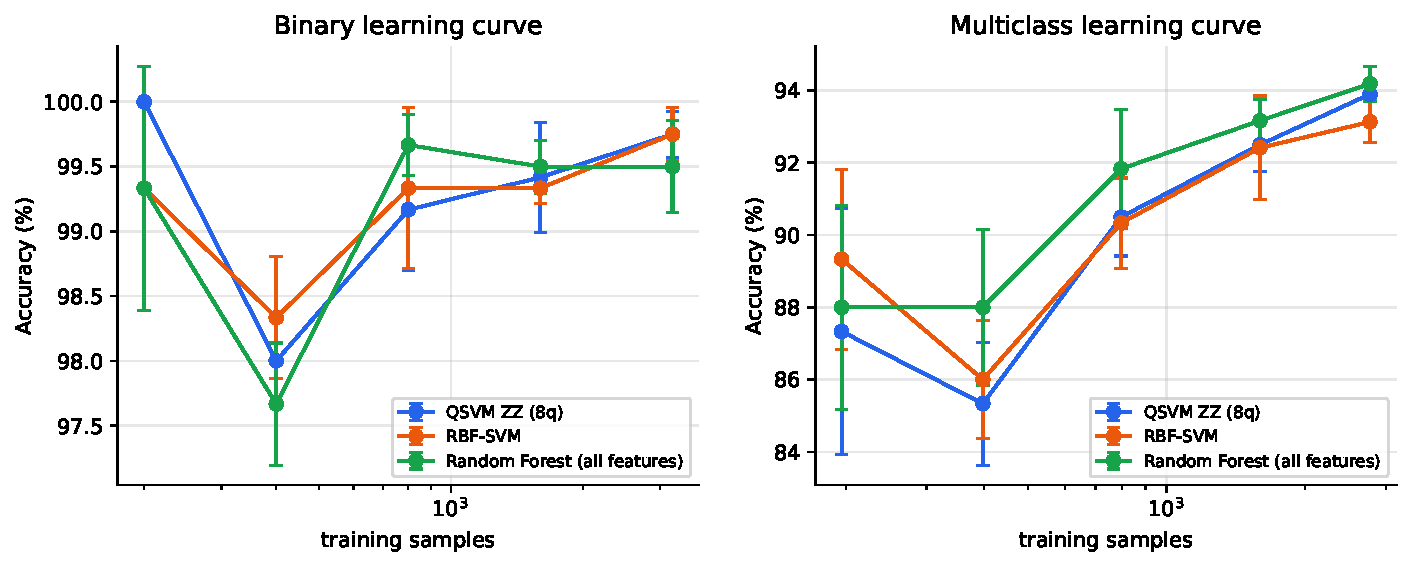
\includegraphics[width=0.95\linewidth]{figures/samples.pdf}
\caption{Accuracy vs.\ number of training flows (8 qubits, 3 seeds). In multiclass mode the
largest setting is capped at 2{,}774 training flows by the 578 unique LDAP flows.}
\label{fig:samples}
\end{figure}

The QSVM and RBF-SVM curves overlap at every size from 200 to 3{,}200 training flows
(Figure~\ref{fig:samples}). Neither model learns faster from few examples, which is sometimes
proposed as an advantage of quantum kernels. Multiclass accuracy is still rising at the largest
size (93.9\% QSVM, 93.1\% RBF-SVM, 94.2\% Random Forest), so more data would help all models, but
deduplication leaves only 578 LDAP flows in this file.

\subsection{Kernel diagnostics}

\begin{table}[H]
\centering\small
\caption{Kernel diagnostics on the training kernel (headline runs, mean over 5 seeds):
off-diagonal mean and standard deviation, centred alignment of the quantum and the tuned RBF
kernel, and the geometric difference $g(K_\text{RBF}\|K_Q)$ on 400 training flows.}
\label{tab:diag}
\resizebox{\linewidth}{!}{%
\begin{tabular}{llccccc}
\toprule
Task & Kernel & Off-diag.\ mean & Off-diag.\ std & Align.\ $K_Q$ & Align.\ $K_\text{RBF}$ & $g(K_\text{RBF}\|K_Q)$ \\
\midrule
binary & ZZ, original ($\alpha{=}1$) & 0.0781 & 0.239 & 0.297 & 0.233 & 65.74 (vs $\sqrt{N}$=20) \\
binary & ZZ, tuned $\alpha$ & 0.0971 & 0.249 & 0.353 & 0.348 & 10.85 (vs $\sqrt{N}$=20) \\
binary & ZZ 16q/2 reps, tuned $\alpha$ & 0.427 & 0.242 & 0.433 & 0.296 & 4.03 (vs $\sqrt{N}$=20) \\
binary & $R_x$, tuned $\alpha$ & 0.294 & 0.267 & 0.370 & 0.296 & 2.90 (vs $\sqrt{N}$=20) \\
\midrule
multiclass & ZZ, original ($\alpha{=}1$) & 0.0701 & 0.23 & 0.494 & 0.479 & 111.97 (vs $\sqrt{N}$=20) \\
multiclass & ZZ, tuned $\alpha$ & 0.0867 & 0.2 & 0.467 & 0.484 & 13.76 (vs $\sqrt{N}$=20) \\
multiclass & ZZ 16q/2 reps, tuned $\alpha$ & 0.084 & 0.218 & 0.487 & 0.484 & 9.19 (vs $\sqrt{N}$=20) \\
multiclass & $R_x$, tuned $\alpha$ & 0.379 & 0.287 & 0.516 & 0.484 & 3.08 (vs $\sqrt{N}$=20) \\

\bottomrule
\end{tabular}}
\end{table}

Table~\ref{tab:diag} explains the results.
\begin{itemize}
\item \textbf{Alignment.} With tuned $\alpha$, the quantum kernels are aligned with the labels about
      as well as the tuned RBF kernel is (binary 0.35--0.43 vs.\ 0.30--0.35; multiclass
      0.47--0.52 vs.\ 0.48). Equal alignment predicts equal accuracy, which is what we observe.
\item \textbf{Geometric difference.} For every tuned quantum kernel, $g$ is well below $\sqrt{N}=20$:
      2.9--3.1 for $R_x$, 4.0--9.2 for the 16-qubit ZZ map and 10.9--13.8 for the paper's ZZ
      settings. By Huang et al.~\cite{huang2021}, a classical kernel trained on the same data can then
      match the quantum kernel's predictions up to a small factor, so no large advantage is
      possible on this data, whatever the labels.
\item \textbf{The original protocol} gives very large $g$ (65.7 binary, 112.0 multiclass). This does
      \emph{not} indicate quantum power: under the original encoding the reference RBF kernel is
      itself badly scaled, and with $\alpha=1$ the quantum kernel is close to the identity, which
      makes \emph{any} smooth kernel look geometrically ``different''. A large $g$ is necessary for
      an advantage, not sufficient, and here the labels do not need the extra geometry.
\end{itemize}

\keybox{Summary of the results}{%
Under a leakage-free protocol with equal tuning, the ZZ quantum-kernel SVM and the classical
RBF-SVM are statistically indistinguishable on every metric, every circuit architecture, every
width from 4 to 16 qubits and every training-set size tested. The original advantages
(+2.15 and +6.85 points) come from duplicate leakage, which mostly helped the QSVM, and from a
linear encoding of heavy-tailed features, which mostly hurt the RBF baseline. A Random Forest
on all raw features is the best model in both tasks.}
